\section{Inhibiting Superpositions with Activations}
\label{sec:act_fns}
The paper presents the activation function as a key in enabling the formation of superpositions in neural nets due to their ability to filter out interference. As such, we demonstrate that modifying the activation function can effectively control the model's usage of superpositions on the same toy model framework as the original paper. 

\subsection{The Extended ReLU Activation}
We propose ExReLU, a modified version of ReLU with the cut-off threshold at $t \in \mathbb{R}$, instead of $0$. By setting $t < 0$, we weaken the filtering effect of the function for negative interference, thus
increasing the 'cost' for the model for adopt superpositional representations.
\[
\text{ExReLU}(x) =
    \begin{cases}
        x & \text{if } x \geq t\\
        0 & \text{if } x < t
    \end{cases}
\] 

\subsection{Model}
We trained two sets of models, each with hidden layers of two neurons on a dataset with five features whilst varying the feature
sparsity. The first model used the normal ReLU activation function, while the second used ExReLU with $t=-0.25$

\subsection{Results}
\begin{figure}[h]
	\centering
	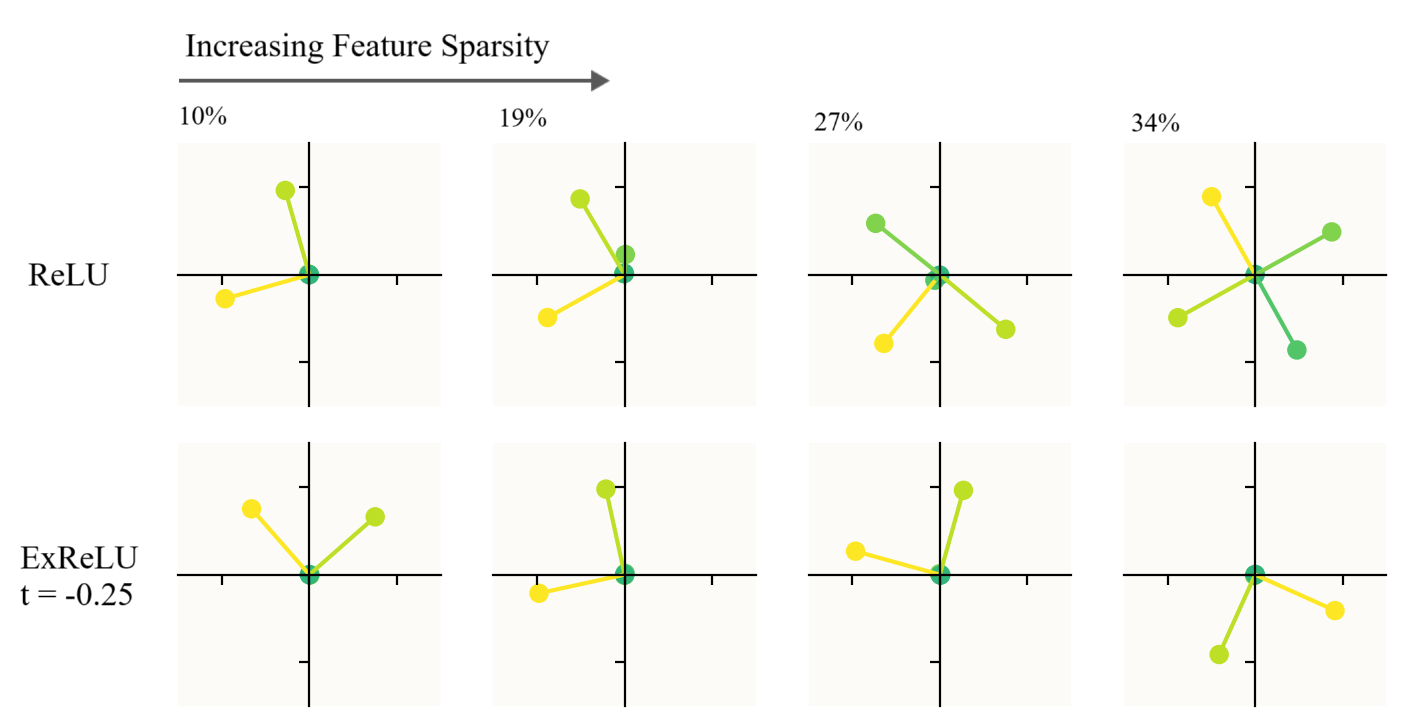
\includegraphics[width=1\linewidth]{figures/acts_diagram.png}
	\caption{Representation of the five features in the hidden layer.}
	\label{fig:acts_diagram}
\end{figure}
Using the \href{https://colab.research.google.com/github/anthropics/toy-models-of-superposition/blob/main/toy_models.ipynb}{toy model framework} to visualize the hidden layer's representation of the features:
Figure \ref{fig:acts_diagram} shows that ExReLU has successfully suppressed the model's usage of superpositions in this instance.
